\section{Tareas de Realizadas en cada Iteración}

Antes de iniciar cada iteración, se sostenía una reunión entre el Dueño del Producto, el \textit{ScrumMaster} y el Pasante, donde se seleccionaban las actividades a realizar durante el \textit{sprint}. Cada actividad se descomponía en tareas y se realizaba un guión sencillo. En la figura \ref{fig:ejemplo_guion} se presenta un guión basado en una actividad realizada en el proceso de desarrollo.


\begin{figure}[h]
	\begin{center}
		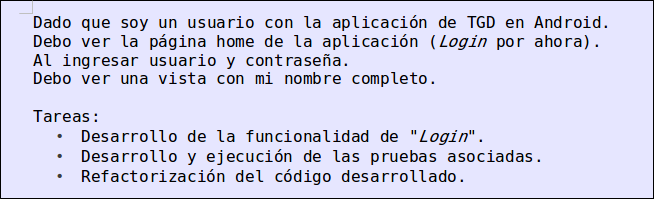
\includegraphics[scale=0.6]{imagenes/guion.png}
	\end{center}
	\caption{
		\label{fig:ejemplo_guion}
		Ejemplo de guión de una actividad a desarrollar
	}
\end{figure}


En las secciones siguientes se realizará una descripción de las tareas realizas, los objetivos planteados en función de las actividades y los resultados obtenidos en cada una de las ocho iteraciones en las que se desarrolló la aplicación móvil. Aunque no esta planteado de forma implícita en los objetivos de cada iteración, en todos los desarrollos se incluye la construcción y ejecución de los casos de prueba.

\subsection{Primera Iteración}

El \textit{sprint} inicial del proyecto consistió en una investigación con el fin de adquirir conocimientos acerca del funcionamiento de las aplicaciones móviles Android, así como de las metodologías y herramientas necesarias para el desarrollo del proyecto. Además fue necesario profundizar en el funcionamiento del API y sus características.

\subsubsection{Objetivos Planteados}
A continuación se enumeran los objetivos planteados:

\begin{itemize}
\item Adquirir conocimientos del funcionamiento y arquitectura del Sistema Operativo Android y de la estructura de las aplicaciones desarrolladas para esta plataforma.
\item Evaluar las herramientas necesarias para el desarrollo del proyecto.
\item Investigar los mecanismos para la aplicación de las metodologías TDD y BDD, en el entorno Android.
\item Analizar las características de cada uno de los servios prestados por el API de Tuguia.de. 
\end{itemize}

\subsubsection{Resultados Alcanzados}

En la sección \ref{subsect:Asociadas_movil} referente a las tecnologías asociadas con la aplicación móvil se expone la información recaudada en esta iteración. Luego de analizarla, se preparó  el entorno de trabajo instalando el IDE en la computadora asignada y se  construyeron varias aplicaciones simples que reafirmaran los conceptos adquiridos.

Para la aplicación de las metodologías se evaluaron varias herramientas entre las que destacan el entorno de pruebas provisto en el SDK y \textit{Robolectric} que es un proyecto de código abierto realizado por terceros.

En el SDK están incluidos todos los elementos necesarios para probar cada aspecto que compone a una aplicación Android, gracias a un entorno de pruebas basado en \textit{JUnit}\footnote{\textit{JUnit:} Es un marco de trabajo para el desarrollo de pruebas sobre aplicaciones Java\cite{JUNIT}}. La ventaja principal de esta herramienta es que al estar embebida no requiere instalar ni aprender ningún complemento externo. Sin embargo, esto trae como desventaja la dependencia de un emulador para su ejecución, lo que retrasa las pruebas en gran medida. \textit{Robolectric} es un marco de trabajo que subsana esta situación, ya que permite simular el entorno Android y ejecutar los casos de prueba directamente en la máquina virtual de Java, no obstante al ser una biblioteca externa implica un aprendizaje extra.

Dadas estas características, se decidió implementar la metodología usando \textit{Robolectric}, ya que se consideró que el tiempo a invertir en aprender la herramienta es inferior al tiempo que se emplearía ejecutando los casos de pruebas en un entorno de trabajo emulado a lo largo de todo el proyecto.

La última fase de esta iteración consistió en el análisis del API de Tuguia.de. Este servicio se encuentra bajo dos capas de seguridad, la primera es una credencial compuesta por un nombre de usuario y una contraseña que deben ser suministrada en la cabecera de cada petición , esto con el objetivo de que el API no pueda ser accedido  por entes externos a la organización. El segundo nivel es la jerarquía de permisos de usuario del sistema de Tuguia.de, de tal forma que un usuario del sistema puede realizar las mismas operaciones tanto en el sitio web como a través del API. 

Al momento de iniciar la pasantía los recursos disponibles eran los siguientes:
\begin{itemize}
\item buscar local: Este servicio se emplea para hacer consultas sobre locales utilizando varios criterios de búsqueda, de no ser utilizado ningún parámetro de búsqueda, se devolverán todos los locales activos de Tuguia.de.
\item buscar comentario: mediante este recurso se pueden obtener los comentarios para uno o mas locales, de no utilizar ningún parámetro de búsqueda, se devolverán todos los comentarios aprobados realizados sobre locales activos de Tuguia.de.
\item buscar taxonomía: A través de esta funcionalidad se obtienen todos los términos de un vocabulario dado dentro de Tuguia.de, por ejemplo, ciudades, categorías, subcategorías, atributos, etc.
\item \textit{user}: Mediante este elemento se accede a las funcionalidades que permiten el manejo de usuarios, específicamente a \textit{login}, \textit{logout} y registro.
\item comentario: Este recurso permite registrar un comentario en Tuguia.de, para su uso es necesario estar conectado como un usuario registrado.
\item local: Este servicio permite agregar locales al sitio. Al igual que en el recurso anterior para su uso es necesario estar conectado como un usuario registrado.
\end{itemize}

Cada uno de estos servicios fue probado y a pesar de funcionar adecuadamente en el caso de éxito, no disponían de un manejo de errores para el resto de los casos. Esta situación debía ser solventada puesto que representaba un gran riesgo para la aplicación móvil, por lo que se decidió investigar un poco más a fondo el funcionamiento del API. Afortunadamente, esta interfaz contaba con una documentación lo suficientemente extensa que permitió familiarizarse con los módulos que lo componían sin dificultad. Gracias a esto se agregó un manejo de errores básico sin alterar la planificación.

Las respuesta del API eran en formato \textit{JSON}\footnote{\textit{JSON:} \textit{JavaScript Object Notation}, es un estándar para el intercambio de datos ligero y legible\cite{JSON}} lo que representó una ventaja gracias a la facilidad existente  para manejar este lenguaje. sin embargo, estas respuestas debían ser ajustadas a la funcionalidad deseada en la aplicación móvil. Este proceso de ajuste se pospuso y se realizó a medida que fue necesario y de esta forma invertir el menor tiempo posible fuera de la aplicación móvil.

\subsection{Segunda Iteración}

Luego del trabajo realizado en la primera iteración, se poseían los elementos necesarios para iniciar el desarrollo de la aplicación móvil, así que se inició con \textit{login}, \textit{logout}, registro y una vista sencilla que permita observar una lista de locales.

\subsubsection{Objetivos Planteados}
En la segunda iteración se plantearon los siguientes objetivos:
\begin{itemize}
\item Desarrollar la funcionalidad de \textit{login} y \textit{logout} para los usuarios registrados.
\item Implementar un mecanismo de registro para los usuarios nuevos.
\item Construir la funcionalidad que permita visualizar una lista de locales. Este mecanismo será usado posteriormente en las búsquedas. 
\end{itemize}


\subsubsection{Resultados Alcanzados}

Por ser esta la primera iteración de desarrollo fue necesario construir un conjunto de funcionalidades secundarias antes de trabajar directamente en los objetivos planteados.

En primer lugar se elaboró un mecanismo \textit{cliente} para realizar peticiones al API que se ajustasen a las políticas de seguridad de este y que pueda recibir las respuestas en el formato JSON. Este mecanismo debe poder ser configurado para generar cualquier tipo de petición.

En segundo lugar se diseñó y construyó un procedimiento para transformar las respuestas provenientes del API a objetos que pudieran ser manejados con mayor facilidad dentro del entorno de la aplicación. Esto fue posible gracias a la biblioteca GSON, que permite transformar un objeto Java en su representación en JSON y viceversa.

Con estas dos herramientas en funcionamiento se desarrollaron los elementos necesarios para alcanzar los objetivos planteados en la iteración siguiendo el esquema presentado en la figura \ref{img:diagrama_flujo} 

\begin{figure}[h]
	\begin{center}
		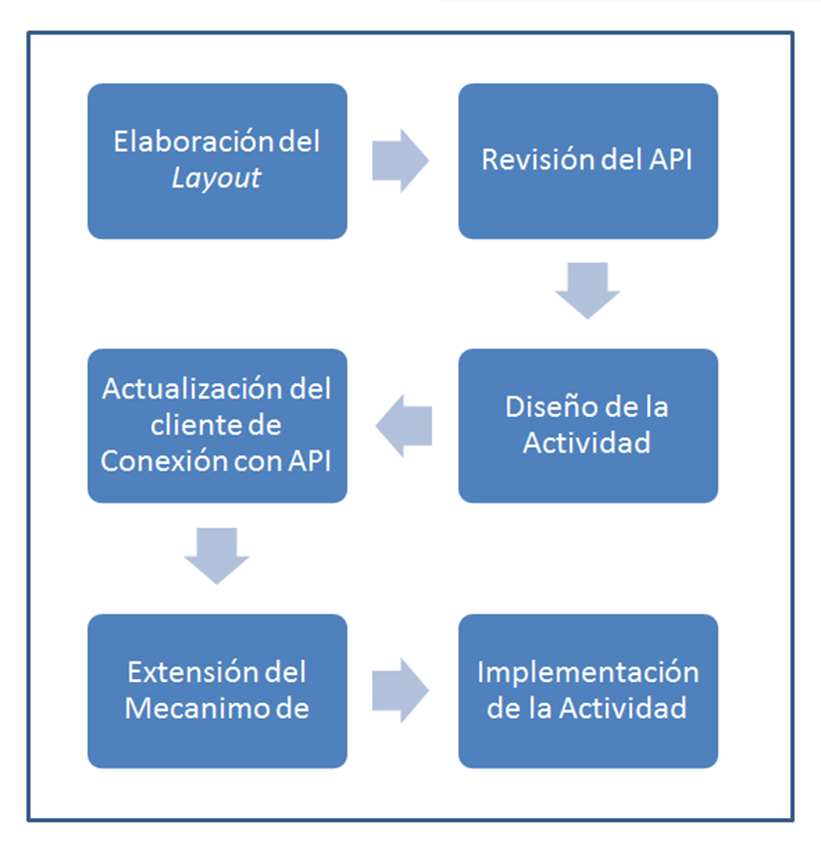
\includegraphics[scale=0.4]{imagenes/diagrama.png}
	\end{center}
	\caption{
		\label{img:diagrama_flujo}
		Esquema de trabajo para el desarrollo de funcionalidades en la aplicación móvil
	}
\end{figure}

\textbf{Diagrama de desarrollo}

En primer lugar se realizó el \textit{layout}, una interfaz sencilla para la funcionalidad en cuestión, no se hace énfasis en la apariencia de éste ya que al finalizar la aplicación, las vistas serán realizadas por el diseñador de Tuguia.de. Luego se revisó a fondo el funcionamiento del servicio del API con el que se iba a interactuar, con el fin de garantizar su correcto funcionamiento. En tercer lugar se realizó el diseño de la actividad que representaría el comportamiento a implementar. Seguidamente se actualizó el mecanismo cliente para poder realizar las peticiones necesarias para este comportamiento y se extendió el procedimiento para traducir las respuestas en formato JSON a objetos Java de acuerdo a las necesidades. Por último se realizó la construcción de la actividad diseñada.

Dadas las características incrementales de la metodología empleada, este flujo de trabajó fue usado repetidamente cada vez que se agregaba una nueva funcionalidad, adaptándolo a las necesidades según el caso y realizando los respectivos casos de prueba.

En el caso del \textit{login} y el registro la funcionalidad se desarrolló sin realizar validaciones de contenido y con un manejo de errores incompleto, es decir, no se realizó un la verficación de los casos de fallo en los que se requiere la participación del usuario. Por otro lado para esta iteración el mecanismo de visualizar la lista de locales construido operaba con una serie de locales simulados sin conectarse a Tuguia.de. Para cada elemento de la lista de locales se muestra la siguiente información: nombre, imagen principal, puntuación, número de comentarios, ciudad, urbanización, subcategoría, si este último atributo no estaba disponible, en su lugar se muestra la categoría. En las figuras 5.4 y 5.5 se puede observar la funcionalidad desarrollada para el \textit{login} y el registro respectivamente.

Un aspecto importante a resaltar es que la información ofrecida de la imagen por el API es el url (\textit{uniform resource locator}); que no es más que la dirección donde se ubica este recurso en Internet. Para acceder a la imagen es necesario realizar una petición a esta dirección para obtenerla. Gracias a este situación y al gran tamaño de las imágenes manejadas en Tuguia.de el consumo de memoria y de la red de datos es bastante alto. Quedó pendiente para futuras iteraciones mejorar esta condición.
 
 
 \begin{figure}
\centering
\begin{minipage}{.5\textwidth}
  \centering
  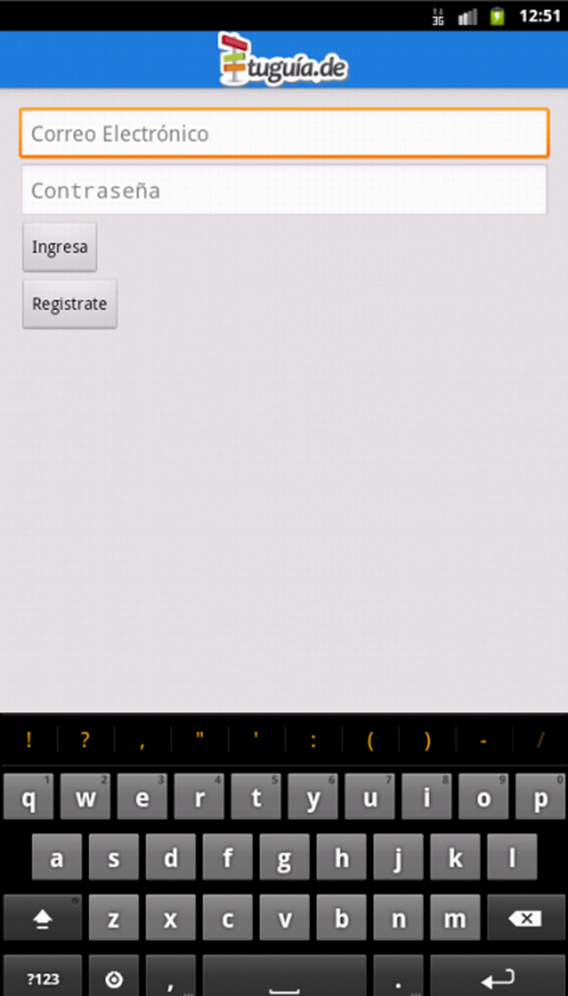
\includegraphics[width=.6\linewidth]{imagenes/login.png}
  \caption{ \textit{Login} en la aplicación móvil}
  \label{fig:login}
\end{minipage}%
\begin{minipage}{.5\textwidth}
  \centering
  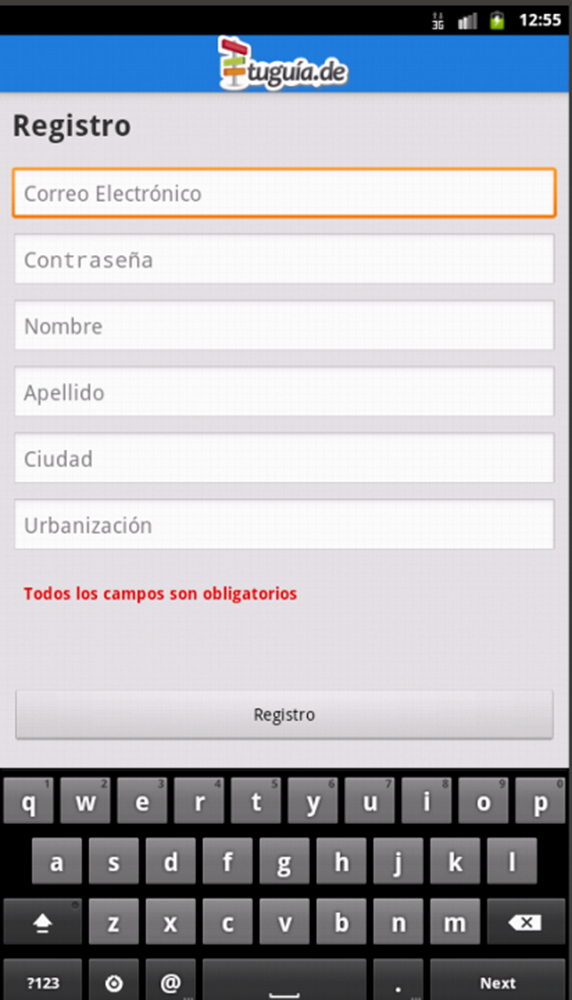
\includegraphics[width=.6\linewidth]{imagenes/login_1.png}
  \caption{Registro de usuarios en la aplicación móvil}
  \label{fig:register}
\end{minipage}
\end{figure}

 
\subsection{Tercera Iteración}

En esta iteración se planteó implementar búsquedas sobre los locales de Tuguia.de dadas una palabra clave y una ubicación. Además se tenía pendiente elaborar el manejo de errores de la iteración anterior.

En este punto del proyecto el módulo del API donde se implementó el manejo de errores, recibió una actualización, por lo que había que instalarla y migrar el manejo de errores como una tarea de mantenimiento.

\subsubsection{Objetivos Planteados} 
En la tercera iteración se plantearon los siguientes objetivos.
\begin{itemize}
\item Actualizar el módulo del API.
\item Migrar el manejo de errores.
\item Desarrollar la funcionalidad que permita realizar búsquedas dada una palabra clave y una ubicación.
\item Completar los casos de fallo pendientes de la iteración dos.
\end{itemize}

\subsubsection{Resultados Alcanzados}

Luego de investigar los mecanismos para la actualización de módulos en Drupal, se hizo un respaldo del sistema y se procedió a actualizar el módulo en cuestión, éste proceso resultó ser bastante automatizado y no presentó mayores inconvenientes. No obstante al inspeccionar el módulo, este había sufrido una refactorización completa, por lo que el proceso de migrar la funcionalidad correspondiente al manejo de errores fue extenso pero se pudo lograr efectivamente.

Para implementar la funcionalidad de búsqueda nuevamente se siguió el esquema de presentando en la figura \ref{img:diagrama_flujo}. Como en el API no existía un mecanismo para realizar búsquedas por  ubicación o coordenadas geográficas, se decidió implementar esta funcionalidad usando solamente palabras claves. Además se integró con el mecanismo de visualizar locales desarrollado en la iteración anterior. El resultado obtenido de esta se muestra en la figura \ref{img:keyword}. El desarrollo necesario para poder realizar las búsquedas dadas una palabra clave y una ubicación o un par de coordenadas se postpuso a una futura iteración.

La funcionalidades pendientes fueron desarrolladas con éxito. 

\begin{figure}[h]
	\begin{center}
		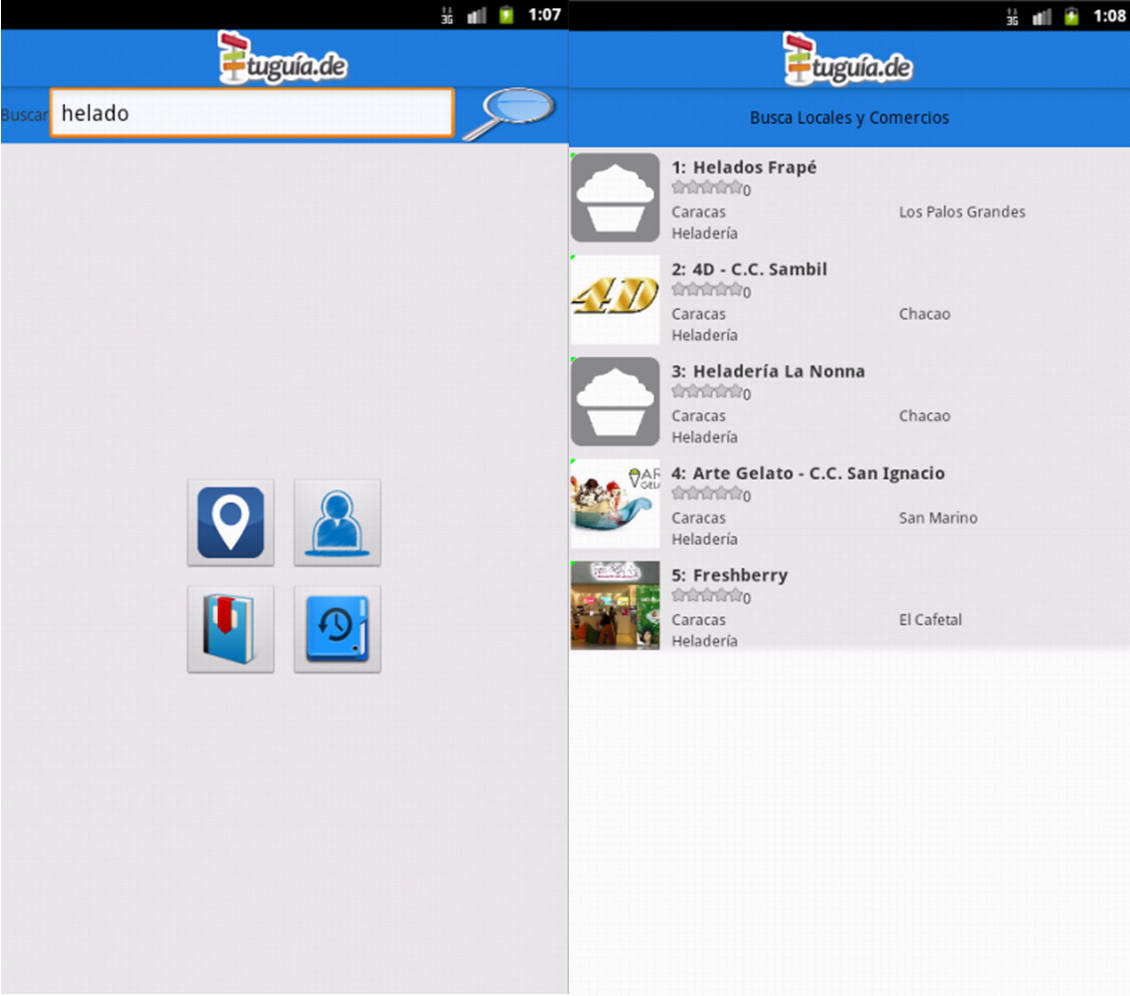
\includegraphics[scale=0.5]{imagenes/search_keyword.png}
	\end{center}
	\caption{
		\label{img:keyword}
		Colaje que muestra la funcionalidad de búsqueda dada una palabra clave
	}
\end{figure}

\subsection{Cuarta Iteración}

En esta iteración se hizo una pausa sobre el desarrollo de la aplicación móvil y se realizó un análisis de la tecnología ApacheSolr y su integración con Drupal dadas las deficiencias encontradas en el \textit{sprint} anterior, con el objetivo de poder extender la funcionalidad del API. 

\subsubsection{Objetivos Planteados} 
A continuación se enumeran los objetivos planteados para la cuarta iteración:
\begin{itemize}

\item Adquirir conocimientos acerca del funcionamiento Apache Solr.
\item Investigar el mecanismo de integración de Drupal y Apache Solr.
\item Implementar la funcionalidad necesaria para realizar búsquedas desde el API, dadas una palabra clave y una ubicación.
\item Desarrollar los mecanismos necesarios para realizar búsquedas desde el API, dadas una palabra clave, unas coordenada geográfica y un radio.

\end{itemize}

\subsubsection{Resultados Alcanzados}

En la sección \ref{subsubsect:solr} referente a las tecnologías asociadas con Tuguia.de se expone la información recaudada en esta iteración acerca de la herramienta Apache Solr. Luego de analizarla, se determinó la manera de incluir la funcionalidad deseada en su comportamiento.

Para implementar la búsqueda por palabra clave y una ubicación se accedió a la configuración del módulo de Drupal que permite integrar Apache Solr al sistema. Mediante la interfaz administrativa de este modulo se agregó un campo de texto llamado ubicación en el documento de configuración de Apache Solr. 

Luego se desarrolló una extensión para este módulo donde se insertó en el campo ubicación, la información contenida, en los atributos ciudad, urbanización y dirección de un local. Cuando se corre el proceso de generación de indices en Apache Solr mediante la interfaz de configuración observado en la figura \ref{img:index_drupal}, el contenido de este campo se segmenta en palabras para que cada una sea tomada como un elemento para la búsqueda.

\begin{figure}[h]
	\begin{center}
		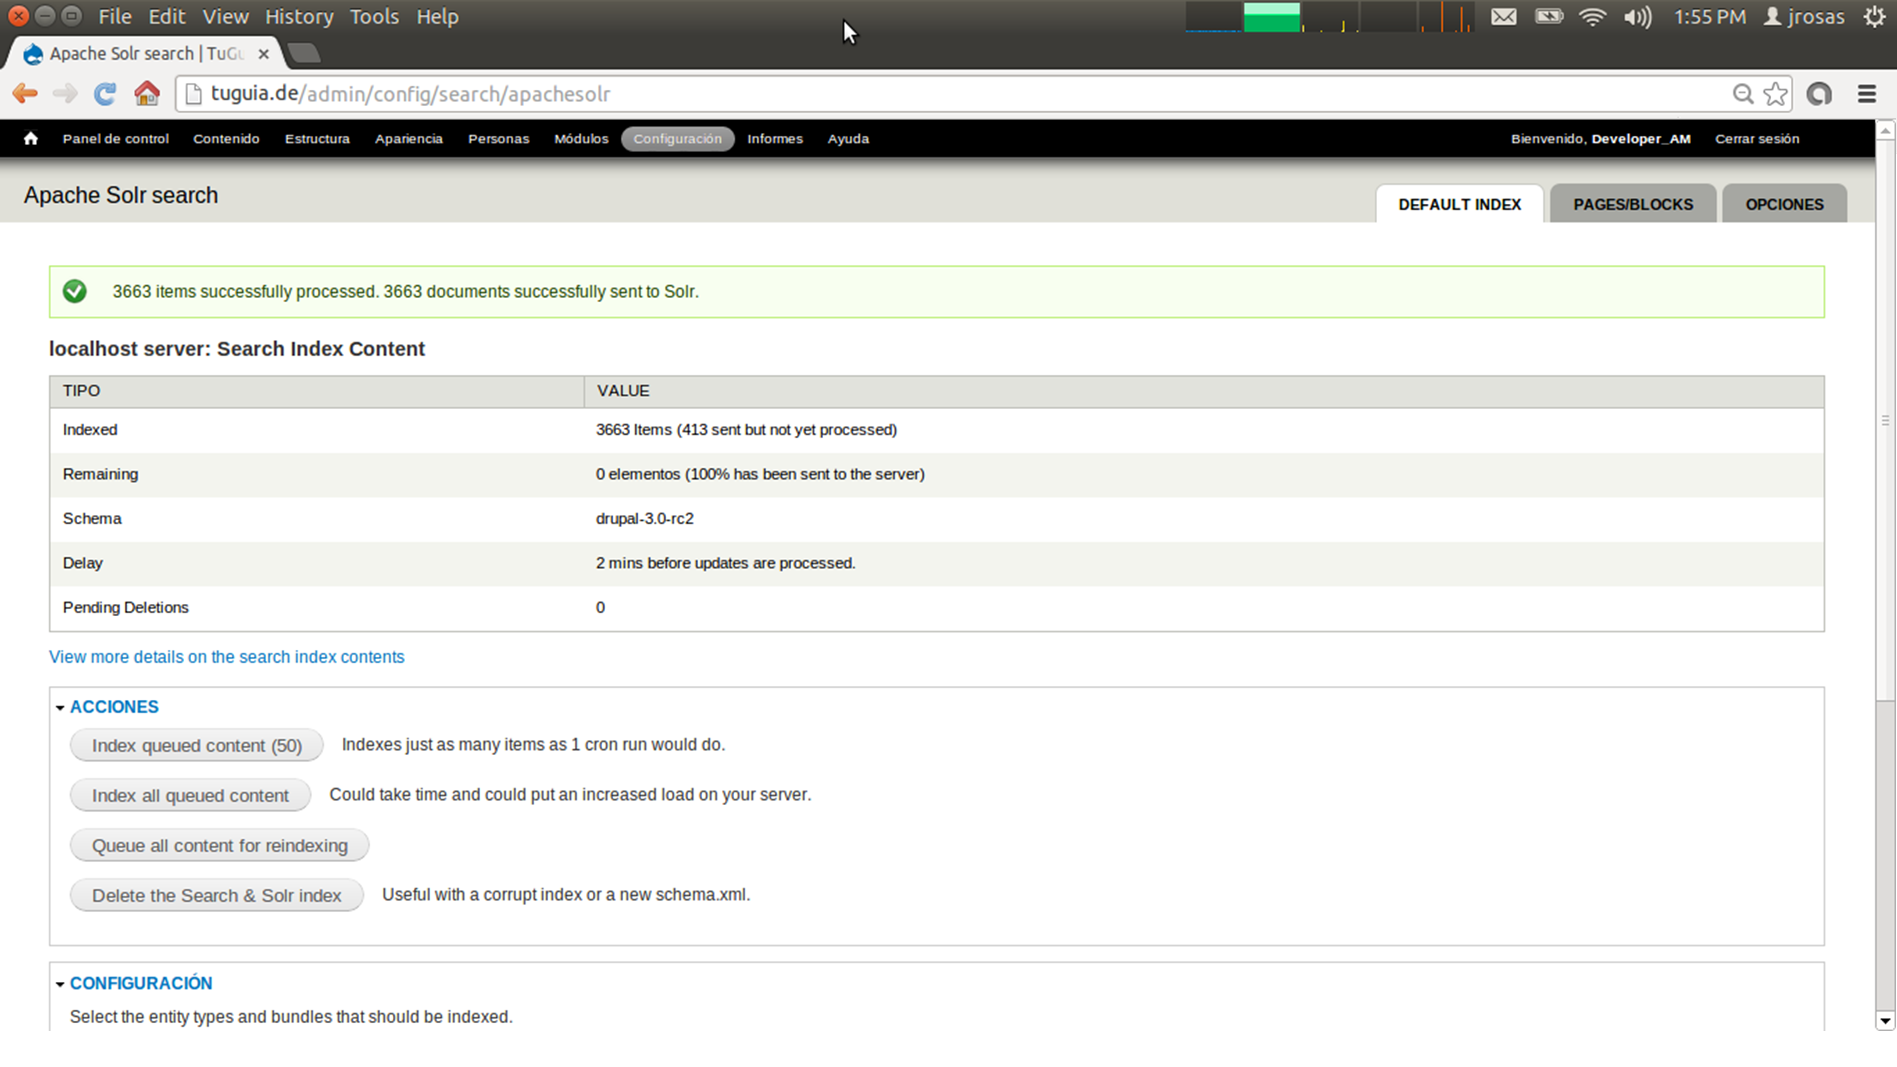
\includegraphics[scale=0.35]{imagenes/solr.png}
	\end{center}
	\caption{
		\label{img:index_drupal}
		Interfaz administrativa del módulo de integración de Drupal con ApacheSolr
	}
\end{figure}

Por último fue necesario agregar un nuevo servicio al API. Para lograr esto se desarrolló y configuró un complemento mediante el cual se hizo posible acceder a la nueva funcionalidad de  búsqueda dada una palabra clave y una ubicación. Por ejemplo al pasar las palabras \textit{pizza} y \textit{Chacao}, se obtienen todos los locales que en algún atributo tenga la palabra pizza y la palabra Chacao en su dirección, ciudad o urbanización.

Como se determinó en la investigación, Apache Solr posee la capacidad para realizar búsquedas dadas un par de coordenadas geográficas. Sin embargo esta funcionalidad no se había configurado en Tuguia.de. Para realizar búsquedas de este tipo fue necesario editar manualmente los archivos de configuración y los documentos de Apache Solr y de esta manera agregar un campo del tipo \textit{location}. Esta configuración se hizo de forma manual y no mediante el módulo de integración como en el caso anterior, debido a que este no presenta soporte para este tipo de campos. 

El proceso seguido a partir de aquí es igual al caso anterior, se agregó la extensión para el módulo de integración de Apache Solr y se agregó un nuevo servicio al API que permite acceder a la funcionalidad.

\subsection{Quinta Iteración}

Con la nueva funcionalidad disponible en el API de \textit{Tuguia.de}, se retoma el desarrollo de la aplicación móvil con el fin de incluir la búsqueda de locales, elemento fundamental de Tuguia.de.
 
\subsubsection{Objetivos Planteados} 
En la quinta iteración se plantearon los siguientes objetivos.
\begin{itemize}

\item Modificar la funcionalidad de búsqueda implementada en la tercera iteración para que adicional a la palabra clave, también reciba ubicación.
\item Implementar la funcionalidad necesaria para realizar búsquedas desde el API, dadas una palabra clave, unas coordenada geográfica y un radio.
\item Desarrollar un mecanismo de paginación para el resultado de las búsquedas.
\end{itemize}

\subsubsection{Resultados Alcanzados}

Como la funcionalidad de búsqueda dada una palabra clave fue implementada en la tercera iteración, en este caso sólo fue necesario modificar el cliente para que usase el nuevo servicio elaborado en la iteración anterior.

En cuanto a la búsqueda por coordenadas, se siguió el flujo de desarrollo planteado en la segunda iteración mostrado en la figura \ref{img:diagrama_flujo}, gracias a este esquema se concluyó con éxito la funcionalidad.

La paginación se implementó modificando el mecanismo para listar locales construido en el segundo \textit{sprint}, de tal forma de que se muestra un máximo de veinte locales por página. Si se realiza una búsqueda con más de veinte locales en el resultado, se listan los veinte primeros y aparece un botón de ``siguientes'' al final de la vista. Al ser pulsado, realiza la petición al API solicitando los veinte siguientes y así sucesivamente hasta mostrar todos los resultados de la búsqueda. Siempre es posible retornar a la página de procedencia pulsando el botón ``anteriores'' que realiza una petición por los locales que corresponden. Este botón es mostrado sólo si se ha avanzado de la primera página. En la figura \ref{img:doblesearch} se ilustra la funcionalidad descrita.
 
\begin{figure}[h]
	\begin{center}
		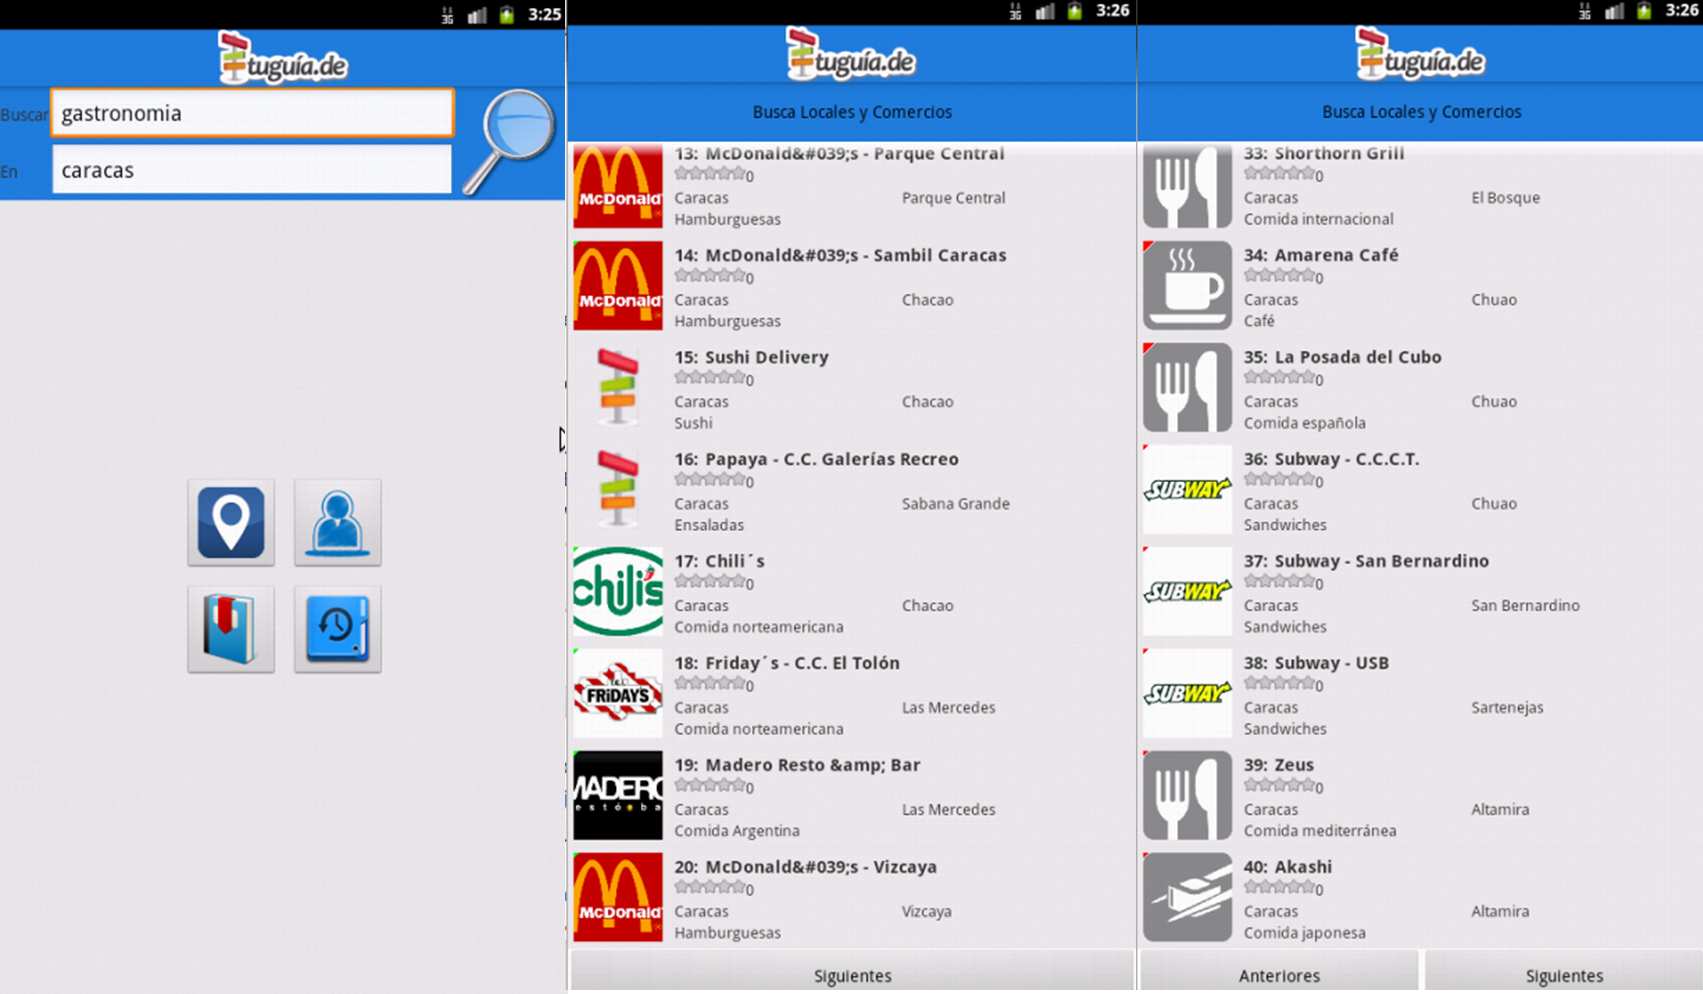
\includegraphics[scale=0.38]{imagenes/search_doble.png}
	\end{center}
	\caption{
		\label{img:doblesearch}
		Colaje que muestra la funcionalidad de búsqueda y de paginado. 
	}
\end{figure}

\subsection{Sexta Iteración}
Continuando con la lista de comportamientos, luego de buscar el local de su preferencia usando los diferentes criterios, la siguiente activad que haría un usuario es ver la información detallada de un local, sus fotografías y los comentarios asociadas a éste. Esas son las tareas que se desarrollaron en esta iteración. 
\subsubsection{Objetivos Planteados} 
En la sexta iteración se establecieron los siguientes objetivos:
\begin{itemize}
\item Implementar una funcionalidad que permite ver información detallada de un local
\item Desarrollar un mecanismo que permita mostrar una lista de comentarios.
\item Construir la funcionalidad que muestre un comentario completo.
\end{itemize}

\subsubsection{Resultados Alcanzados}

Para la implementación de estas tres funcionalidades se siguió el flujo de desarrollo empleado en las iteraciones anteriores (figura \ref{img:diagrama_flujo}) y en los tres casos se lograron desarrollar con éxito. A continuación se detallan los aspectos mas relevantes del desarrollo.

En la vista detallada de un local mostrada en la figura 5.9, se muestra la siguiente información: nombre, puntuación, número de comentarios, las categorías a las que pertenece, un botón con el número de teléfono que funciona como un acceso directo, al presionarlo lleva directamente a la aplicación usada para hacer llamadas marcando este número y la dirección. Ademas en este \textit{layout} se muestra una lista de cinco comentarios realizados sobre el local y un botón de ver todos los comentarios, que lleva a otra pantalla donde se muestra la lista completa.

En Tuguia.de no existe un límite para la longitud de la reseña de un usuario, por lo que en las listas de comentarios, se acotó el texto de la descripción a dos lineas. Si se presiona sobre un comentario, se va a una vista que muestra el contenido completo tal y como es mostrado en la figura 5.10.

 \begin{figure}
\centering
\begin{minipage}{.5\textwidth}
  \centering
  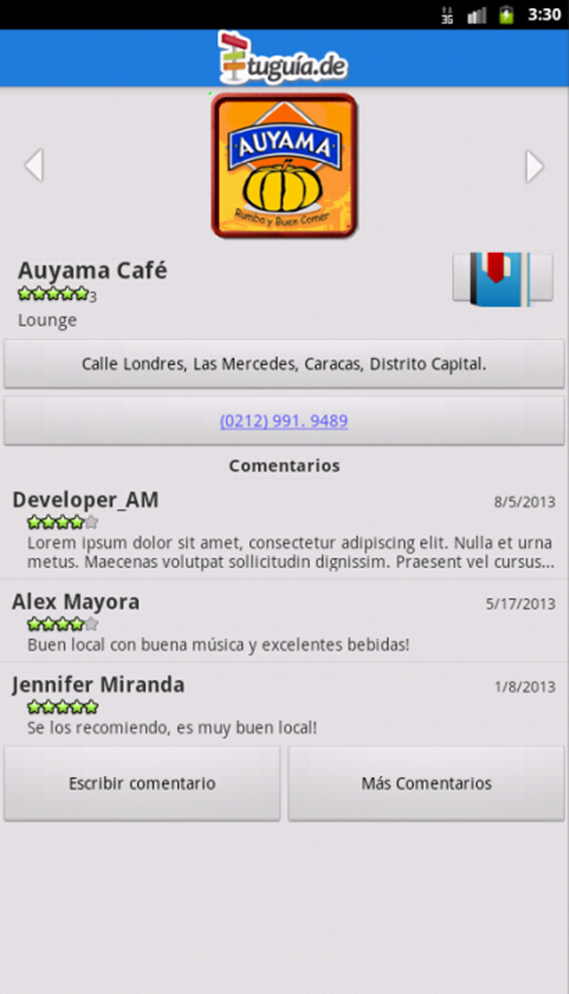
\includegraphics[width=.6\linewidth]{imagenes/detalle.png}
  \caption{Vista detallada de un local}
  \label{fig:detalle_local}
\end{minipage}%
\begin{minipage}{.5\textwidth}
  \centering
  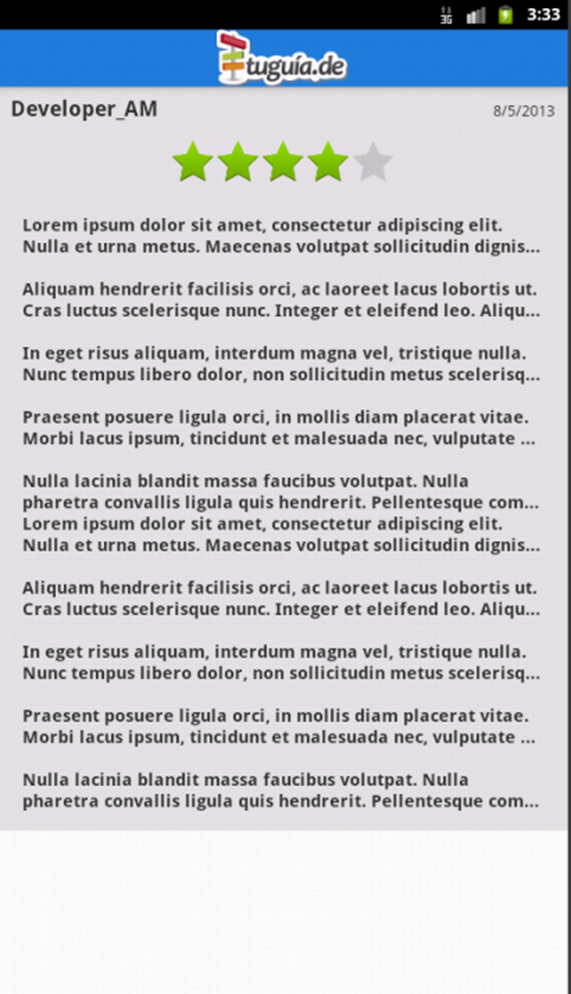
\includegraphics[width=.6\linewidth]{imagenes/comentario_completo.png}
  \caption{Vista de un comentario completo}
  \label{fig:comentario_full}
\end{minipage}%

\end{figure}

\subsection{Séptima Iteración}

En esta iteración se realizó un desarrollo orientado al manejo de las bases de datos internas de la aplicación, con el fin de registrar los usuarios y los locales vistos. De esta manera poder ofrecer un registro de los locales vistos recientemente por el usuario y la posibilidad de almacenar los locales favoritos, además de un manejo de sesión para el usuario en la aplicación.

\subsubsection{Objetivos Planteados} 
A continuación se enumeran los objetivos establecidos:
\begin{itemize}
\item Crear el modelo de datos necesario para almacenar locales y usuarios en una base de datos de la aplicación
\item Construir la funcionalidad que permita almacenar automáticamente los locales recientemente vistos por el usuario.
\item Implementar la funcionalidad para que los usuarios pueden almacenar sus locales favoritos.
\item Desarrollar un manejo de sesión para que una instancia de la aplicación pueda ser usada por múltiples usuarios. 
\end{itemize}

\subsubsection{Resultados Alcanzados}

Gracias a la base de datos SQLite embebida dentro del sistema operativo Android, se disponía de todos los elementos necesarios para almacenar los locales. Se tomó la decisión de crear dos tablas independientes, una para almacenar los locales vistos recientemente y la segunda para los favoritos del usuario, a pesar que ambas manejan los mismos atributos.

Esta decisión fue tomada para facilitar el manejo de las operaciones sobre las tablas, ya que a pesar de que manejan la misma información el comportamiento es distinto. Con esta elección se buscaba también minimizar el tamaño de la base de datos. En una sola tabla se hubiese requerido una columna extra que identificase los locales recientes y los favoritos. Esta columna adicional a la larga podría representar mas espacio que el costo por mantener dos tablas separadas.

Cuando se visualiza la información detallada de un local, éste es agregado en la tabla creada para almacenar los locales recientes automáticamente. Ademas en este \textit{layout} se dispuso de un botón que permite que el usuario identifique un local como favorito. Para que tener acceso a esta funcionalidad los usuarios deben haber sido autentificados pasando exitosamente por el proceso de \textit{login}. De esta forma todos los locales almacenados en la aplicación son marcados con un identificador único correspondiente al usuario autentificado que esté usando la aplicación en ese momento. 

Otro aspecto importante de la gestión de sesión que se implementó fue el manejo de \textit{cookies}\footnote{\textit{Cookies}: pequeños fragmentos de información enviados al servidor en cada petición realizada} ya que este mecanismo permite que no sólo se esté autentificado en la aplicación móvil, sino que también a través del envío de un identificador único de usuario en un \textit{cookie}, se puede interactuar con el sitio web como si éste se hubiera autentificado.

\subsection{Octava Iteración}

La última iteración se enfocó en mejorar la eficiencia del manejo de recursos en la aplicación y de agregar la funcionalidad que permite realizar comentarios en Tuguia.de.

\subsubsection{Objetivos Planteados} 
Los objetivos planteados en esta iteración fueron los siguientes:
\begin{itemize}
\item Diseñar e implementar la funcionalidad que permita subir comentarios asociados a un local de Tuguia.de.
\item Implementar diferentes mecanismos que permitan que la aplicación realice el menor uso posible de la red de datos
\end{itemize}

\subsubsection{Resultados Alcanzados}

La funcionalidad correspondiente a los comentarios siguió el esquema planteado y fue desarrollada sin problema. Este comportamiento solo esta disponible una vez que el usuario esta autentificado y se puede acceder a él, a través de la vista detallada de un local. Este mecanismo se muestra en la figura \ref{img:comentario}

\begin{figure}[h]
	\begin{center}
		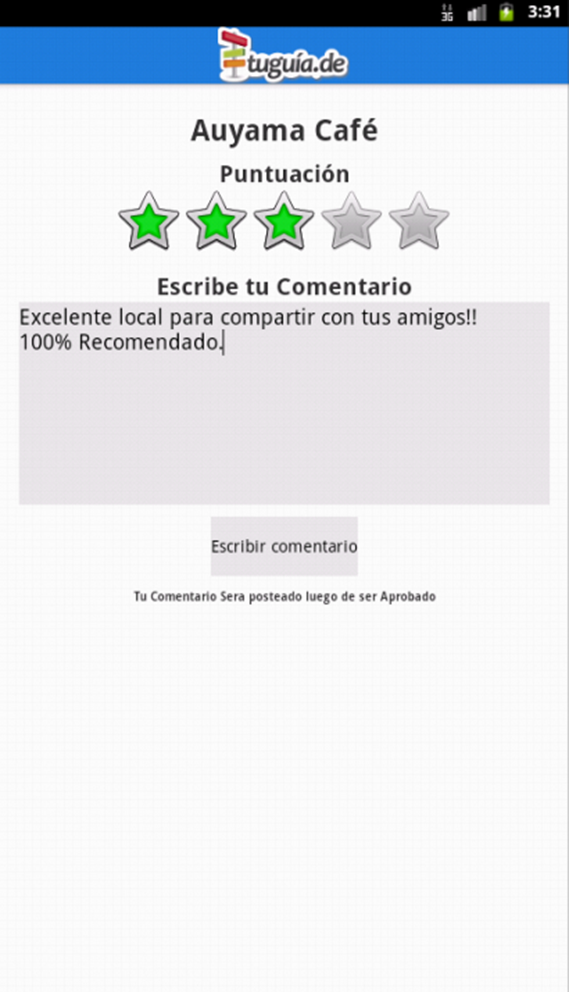
\includegraphics[scale=0.4]{imagenes/escribir_coment.png}
	\end{center}
	\caption{
		\label{img:comentario}
		Interfaz para escribir comentarios en Tuguia.de.
	}
\end{figure}


A lo largo del desarrollo de la aplicación se idearon diversos mecanismos que permitieron optimizar no sólo el uso de la red, si no que también la memoria que consume la aplicación en ejecución.

La primera mejora es la integración de la biblioteca de manejo de imágenes \textit{Picasso}, que ofrece la posibilidad de realizar diversas transformaciones de imágenes. Gracias a esto es posible reducir el tamaño de las imágenes recibidas, de tal forma que el espacio ocupado en memoria sea el menor. Además provee un mecanismo de soporte a fallas, cada petición es intentada tres veces antes de descartar el recurso. Si el recurso es descartado, se coloca una imagen por defecto y de esta forma no se dejan espacios vacíos en la interfaz. Por último, permite implementar mecanismos de caché en la memoria del teléfono, de esta forma cuando se descarga una imagen, una copia es guardada en la memoria. Si por cualquier razón la aplicación intenta descargar nuevamente la misma imagen se retorna la copia que se encuentra en memoria. Como se mencionó anteriormente, las imágenes manejadas en Tuguia.de son de gran tamaño, la suma de los elementos brindados por ésta librería (ajuste de tamaño, caché y soporte de fallos) representó una cambió considerable en el funcionamiento de la aplicación. 

Por otro lado se modificó también el comportamiento del paginado, buscando reducir el uso de la red de datos. Se implementó un mecanismo para guardar en archivos de texto las páginas de resultado. De esta forma al moverse entre las páginas, se verifica si existe un archivo que la contenga, antes de hacer una petición al API para obtenerla. Este enfoque no es solo mas eficiente sino que permite un desplazamiento más fluido dentro de la aplicación.

Como última mejora se editaron las respuestas del API para cada recurso eliminando todos los campos que no eran necesarios en la aplicación móvil. De esta forma en cada petición sólo se obtiene la información que es necesaria para mantener  al mínimo la cantidad de información transferida por la red.




